\section*{Problem B}\label{sec:experimental}

\textit{Select the spiral pattern for the data.}
\begin{itemize}
    \item \textit{Using all the features available, find a solution that fits the training data. What training and test error do
    you achieve? Is this a low bias/high variance or high bias/low variance model? How do you know?}

    \item \textit{Using only (x1, x2), find a solution that fits the training data. What training and test error do you achieve?
    Is this a low bias/high variance or high bias/low variance model? How do you know?}


\end{itemize}
\textit{For both solutions, detail your hyperparameter choices by providing a screenshot and the URL to your
solution (the URL contains all your settings choices).}


A low bias/high vairance model typically fits the traning data very well, but is not so robust with unkown test data. This is typically due to overfitting with too many parameters. On the contrary, a high bias/low variance model usually fits the training and test data equally poorly. This can be due to a model that is not complex enough to capture the trend of the data. 

With complete freedom, a neural network using the ReLU activation and $x_1,x_2,x_1^2,x_2^2, x_1x_2, \sin(x_1),\sin(x_2)$ as features was used. The final model contained 2 hidden layers each with 8 neurons as shown in Figure \ref{fig:spiral_all}. After 792 epochs, a training and test loss of 0.002 and 0.031 was obtained, respectfully. Thus, it can be said that this is a high varience/low bias model.

The neural network constrained to using only $x_1,x_2$ as features is shown in Figure \ref{fig:spiral_x1_x2}. It consists of 3 hidden layers each with 8 neurons. After 822 epochs, a the training and test losses were 0.001 and 0.029, respectfully. Again, this points to the model being a low  bias/high vareiance model.

\begin{figure}[htbp]
    \centering
    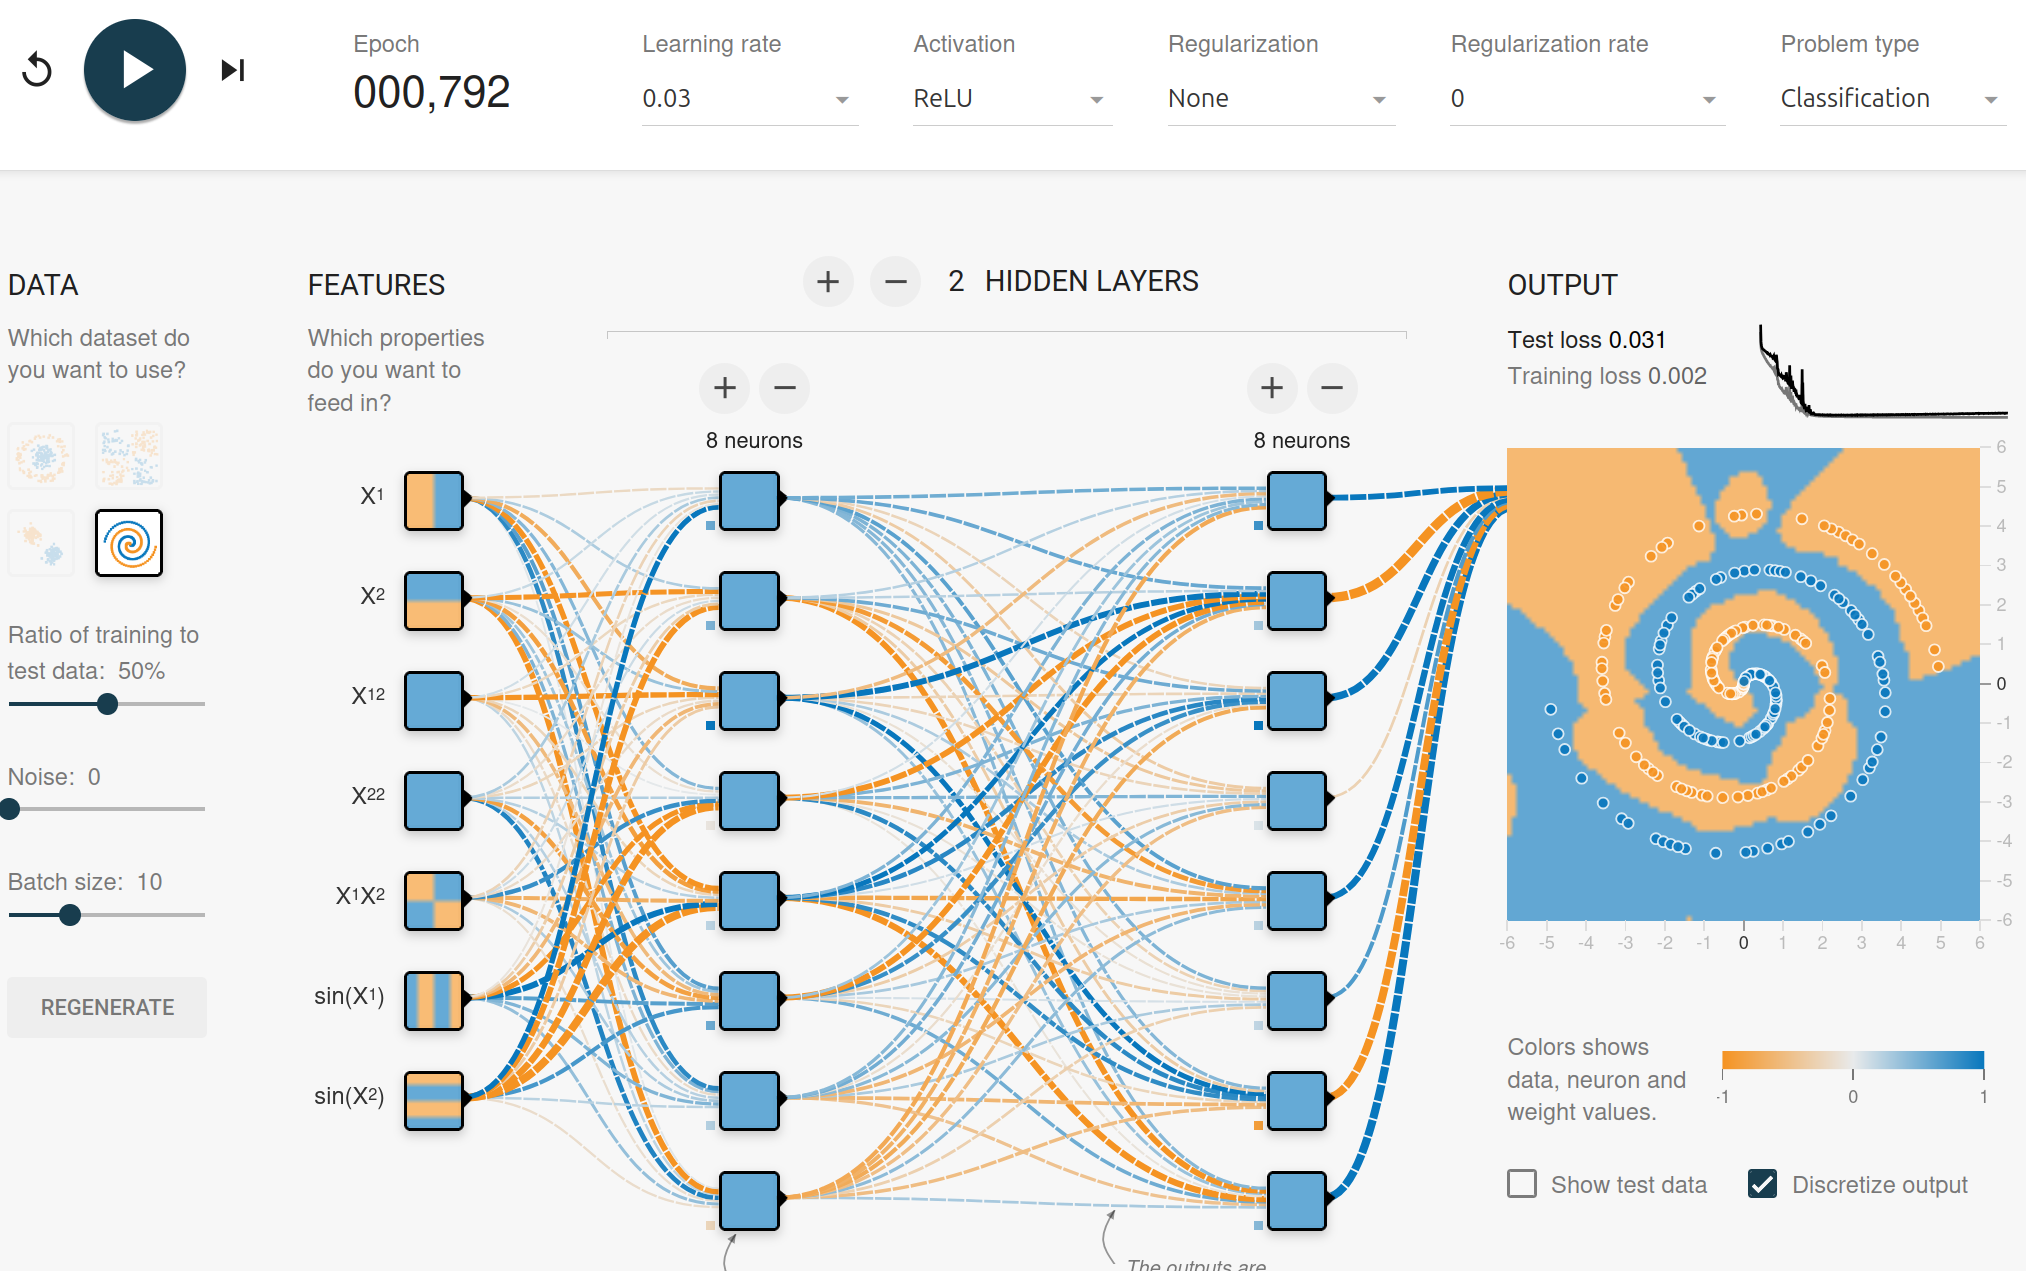
\includegraphics[width = 0.9\linewidth]{img/spiral_all.png}
    \caption{The neural network obtained with complete freedom.}
    \label{fig:spiral_all}
\end{figure}
\begin{figure}[htbp]
    \centering
    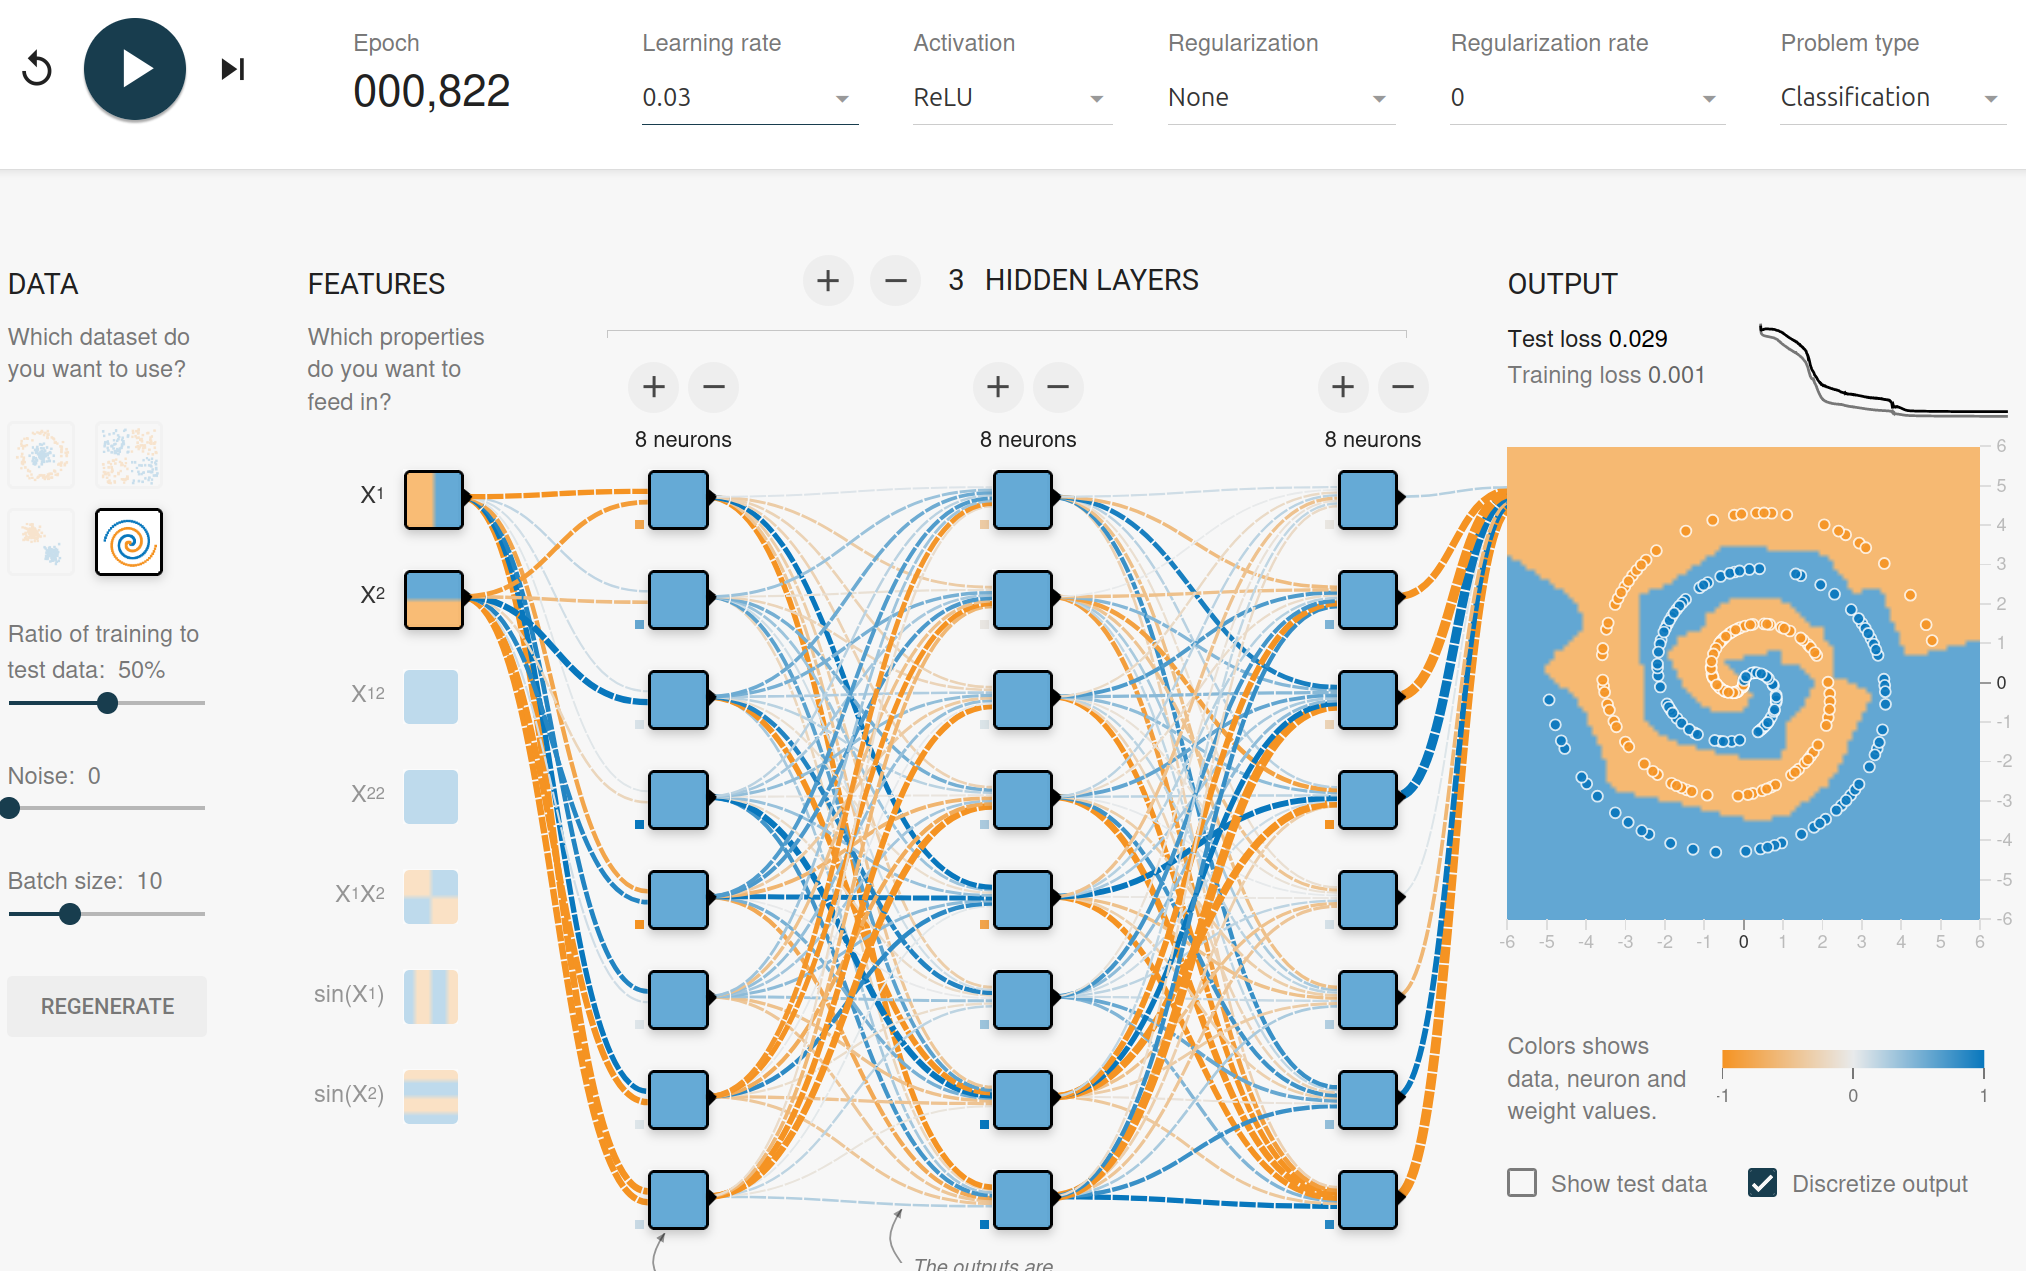
\includegraphics[width = 0.9\linewidth]{img/spiral_x1_x2.png}
    \caption{The neural network obtained with the features constrained to $x_1$ and $x_2$. }
    \label{fig:spiral_x1_x2}
\end{figure}

